\section{Casi d'uso}
\subsection{Attori dei casi d'uso}
\begin{figure}[H]
\centering
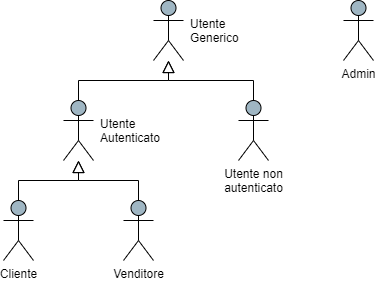
\includegraphics[scale=0.6]{res/UseCase/Immagini/DiagrammaAttoriPrimari}
\caption{Diagramma UML\ped{G} per la gerarchia degli attori primari}
\end{figure}
\subsubsection{Attori primari}
\begin{itemize}
\item \textbf{Utente generico:} corrisponde ad un utente generico che accede alla piattaforma attraverso l'applicazione Web\ped{G};
\item \textbf{Utente autenticato:} corrisponde ad un utente che ha effettuato la procedura di login per autenticarsi. L'utente risulta quindi in possesso delle credenziali valide per accedere ad apposite funzionalità;
\item \textbf{Utente non autenticato:} corrisponde ad un utente che non ha ancora effettuato la procedura di login alla piattaforma;
\item \textbf{Cliente:} corrisponde ad un utente che ha la possibilità di acquistare i prodotti presenti nel catalogo digitale;
\item \textbf{Venditore:} corrisponde all'utente che possiede la piattaforma, in quanto ha la possibilità vendere e gestire i propri prodotti presenti nell'applicativo;
\end{itemize}
\subsubsection{Attori secondari}
\begin{itemize}
\item \textbf{Stripe\ped{G}:} infrastruttura software che fornisce i servizi di pagamento necessari agli acquisti nella piattaforma;
\item \textbf{AWS Cognito\ped{G}:} Identity Manager, offre un servizio di gestione delle identità per custodire le credenziali degli utenti in un cloud\ped{G} esterno.
\end{itemize}
\subsection{Elenco dei casi d'uso}
In questa sezione vi sono elencati tutti i casi d'uso (UC) individuati. Ogni UC rappresenta uno scenario per uno o più attori e viene descritto tramite diagrammi dei casi d'uso. Ogni UC, infine, possiede una precondizione e una postcondizione. \\

\begin{figure}[H]
\centering
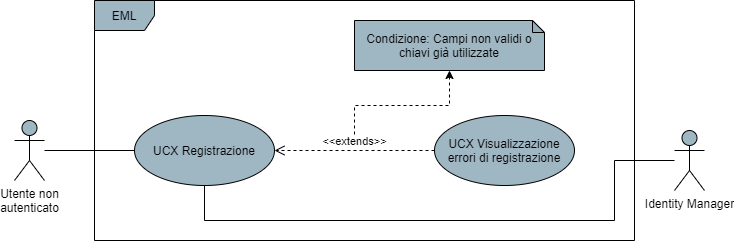
\includegraphics[scale=0.6]{res/UseCase/Immagini/RegistrazioneGenerale}
\caption{Diagramma UML per modulo di registrazione}
\end{figure}

\subsubsection{UC1 - Registrazione}
\begin{itemize}
\item \textbf{Attori primari}: utente non autenticato;
\item \textbf{Attori secondari}: Identity Manager;
\item \textbf{Descrizione}: viene effettuata la registrazione nel sistema, inserendo i propri dati personali nella pagina dedicata;
\item \textbf{Scenario Principale}: l'utente non autenticato accede alla pagina di registrazione, il sistema rende disponibili i campi da compilare, l'utente compila i campi [\textbf{UC1.1}], conferma la registrazione [\textbf{UC1.2}] e l'Identity Manager si occupa della registrazione nel sistema;
\item \textbf{Estensioni}:
\begin{itemize}
\item \textbf{UC2}: se i campi non sono validi o l'email è già stata utilizzata nel sistema, viene mostrato un errore di registrazione all'utente non autenticato e l'utente potrà provare nuovamente ad eseguire la registrazione.
\end{itemize}
\item \textbf{Precondizione}: l'utente non autenticato intende registrarsi nel sistema come cliente;
\item \textbf{Postcondizione}: l'utente risulta registrato nel sistema come cliente.
\end{itemize}

\begin{figure}[H]
\centering
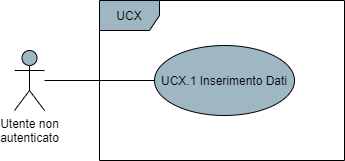
\includegraphics[scale=0.6]{res/UseCase/Immagini/Registrazione}
\caption{Diagramma UML per UC1 - Registrazione}
\end{figure}

\subsubsection{UC1.1 - Inserimento dati}
\begin{itemize}
\item \textbf{Attori primari}: utente non autenticato;
\item \textbf{Descrizione}: l'utente compila il form per la registrazione nel sistema;
\item \textbf{Scenario Principale}: l'utente inserisce i seguenti dati personali:
\begin{itemize}
\item nome [\textbf{UC1.1.1}];
\item cognome [\textbf{UC1.1.2}];
\item indirizzo di fatturazione [\textbf{UC1.1.3}];
\item email [\textbf{UC1.1.4}];
\item password [\textbf{UC1.1.5}].
\end{itemize}
\item \textbf{Precondizione}: l'utente non autenticato è all'interno della pagina di registrazione;
\item \textbf{Postcondizione}: l'utente ha compilato tutti campi e può procedere alla registrazione.
\end{itemize}

\begin{figure}[H]
\centering
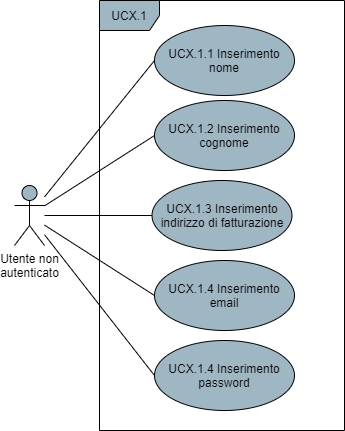
\includegraphics[scale=0.6]{res/UseCase/Immagini/InserimentoDatiRegistrazione}
\caption{Diagramma UML per UC1.1 - Inserimento dati}
\end{figure}


\subsubsection{UC1.1.1 - Inserimento nome}
\begin{itemize}
\item \textbf{Attori primari}: utente non autenticato;
\item \textbf{Descrizione}: l'utente deve compilare il campo "Nome" per procedere alla registrazione;
\item \textbf{Scenario Principale}: l'utente inserisce il suo nome nell'apposito campo;
\item \textbf{Precondizione}: il campo "Nome" risulta vuoto;
\item \textbf{Postcondizione}: il campo "Nome" è stato compilato.
\end{itemize}

\subsubsection{UC1.1.2 - Inserimento cognome}
\begin{itemize}
\item \textbf{Attori primari}: utente non autenticato;
\item \textbf{Descrizione}: l'utente deve compilare il campo "Cognome" per procedere alla registrazione;
\item \textbf{Scenario Principale}: l'utente inserisce il suo cognome nell'apposito campo;
\item \textbf{Precondizione}: il campo "Cognome" risulta vuoto;
\item \textbf{Postcondizione}: il campo "Cognome" è stato compilato.
\end{itemize}

\subsubsection{UC1.1.3 - Inserimento indirizzo di fatturazione}
\begin{itemize}
\item \textbf{Attori primari}: utente non autenticato;
\item \textbf{Descrizione}: l'utente deve compilare il campo "Indirizzo di fatturazione" per procedere alla registrazione;
\item \textbf{Scenario Principale}: l'utente inserisce il suo indirizzo di fatturazione nell'apposito campo;
\item \textbf{Precondizione}: il campo "Indirizzo di fatturazione" risulta vuoto;
\item \textbf{Postcondizione}: il campo "Indirizzo di fatturazione" è stato compilato.
\end{itemize}

\subsubsection{UC1.1.4 - Inserimento email}
\begin{itemize}
\item \textbf{Attori primari}: utente non autenticato;
\item \textbf{Descrizione}: l'utente deve compilare il campo "Email" per procedere alla registrazione;
\item \textbf{Scenario Principale}: l'utente inserisce la sua email nell'apposito campo;
\item \textbf{Precondizione}: il campo "Email" risulta vuoto;
\item \textbf{Postcondizione}: il campo "Email" è stato compilato.
\end{itemize}

\subsubsection{UC1.1.5 - Inserimento password}
\begin{itemize}
\item \textbf{Attori primari}: utente non autenticato;
\item \textbf{Descrizione}: l'utente deve compilare il campo "Password" per procedere alla registrazione;
\item \textbf{Scenario Principale}: l'utente inserisce una password nell'apposito campo;
\item \textbf{Precondizione}: il campo "Password" risulta vuoto;
\item \textbf{Postcondizione}: il campo "Password" è stato compilato.
\end{itemize}

\subsubsection{UC1.2 - Conferma registrazione}
\begin{itemize}
\item \textbf{Attori primari}: utente non autenticato;
\item \textbf{Descrizione}: l'utente conferma i dati presenti nel form e si registra nel sistema;
\item \textbf{Scenario Principale}: l'utente preme il tasto di conferma di registrazione e manda la richiesta al sistema per la registrazione di un account con i dati presenti nel form;
\item \textbf{Precondizione}: l'utente non autenticato si trova all'interno della pagina di registrazione;
\item \textbf{Postcondizione}: la richiesta di registrazione è stata mandata al sistema.
\end{itemize}

\subsubsection{UC2 - Visualizzazione errori di registrazione}
\begin{itemize}
\item \textbf{Attori primari}: utente non autenticato;
\item \textbf{Descrizione}: l'utente non autenticato visualizza un errore riguardante i campi di registrazione che ha inserito. Questi errori possono essere:
\begin{itemize}
\item \textbf{Campo non valido}: un campo risulta vuoto o con caratteri non validi;
\item \textbf{Email già utilizzata}: l'email è già stata utilizzata da un altro cliente.
\end{itemize}
\item \textbf{Scenario Principale}: il sistema riconosce uno o più errori nei campi inseriti dall'utente e vengono visualizzati nella pagina di registrazione;
\item \textbf{Precondizione}: l'utente non autenticato ha inserito i campi ed ha provato ad effettuare la registrazione;
\item \textbf{Postcondizione}: viene visualizzato un messaggio di errore nella pagina di registrazione e l'utente non risulta autenticato nel sistema.
\end{itemize}


\begin{figure}[H]
\centering
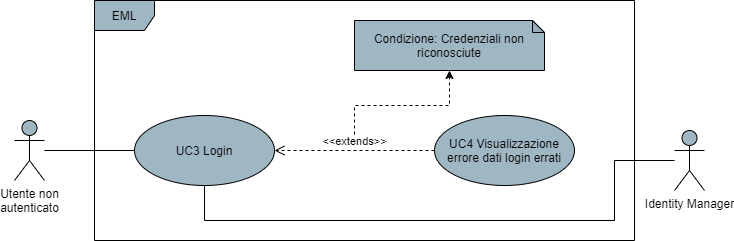
\includegraphics[scale=0.6]{res/UseCase/Immagini/Login}
\caption{Diagramma UML per modulo di login}
\end{figure}

\subsubsection{UC3 - Login}
\begin{itemize}
\item \textbf{Attori primari}: utente non autenticato;
\item \textbf{Attori secondari}: identity manager;
\item \textbf{Descrizione}: l'utente, inserendo le proprie credenziali, viene autenticato alla piattaforma;
\item \textbf{Scenario Principale}: l'utente non ancora autenticato seleziona il tipo di utente \textbf{[UC3.1]}, inserisce le proprie credenziali negli appositi campi dati \textbf{[UC3.2]} e richiede il login \textbf{[UC3.3]};
\item \textbf{Estensioni}:
\begin{itemize}
	\item \textbf{UC4}: se le credenziali inserite non vengono riconosciute dall'identity manager, viene visualizzato un messaggio che informa l'utente dell'errore;
\end{itemize}
\item \textbf{Precondizione}: l'utente prova ad autenticarsi alla piattaforma;
\item \textbf{Postcondizione}: l'utente viene autenticato come il tipo di utente selezionato in \textbf{[UC3.1]}.
\end{itemize}

\begin{figure}[H]
\centering
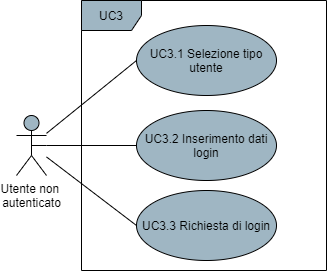
\includegraphics[scale=0.6]{res/UseCase/Immagini/LoginSottocasi}
\caption{Diagramma UML per UC3 - Login}
\end{figure}

\subsubsection{UC3.1 - Selezione tipo utente}
\begin{itemize}
\item \textbf{Attori primari}: utente non autenticato;
\item \textbf{Descrizione}: l'utente seleziona il tipo di utente per effettuare il login;
\item \textbf{Scenario Principale}: l'utente indica se vuole effettuare il login come cliente o come venditore;
\item \textbf{Precondizione}: il form di inserimento dati per selezione del tipo di utente è disponibile;
\item \textbf{Postcondizione}: è stato selezionato il tipo di utente per il login.
\end{itemize}

\subsubsection{UC3.2 - Inserimento dati login}
\begin{itemize}
\item \textbf{Attori primari}: utente non autenticato;
\item \textbf{Descrizione}: l'utente compila il form per il login;
\item \textbf{Scenario Principale}: l'utente inserisce nel form apposito i dati necessari al login;
\item \textbf{Specializzazioni}: a seconda del tipo di utente selezionato in \textbf{[UC3.1]}
\begin{itemize}
	\item inserimento dati login cliente \textbf{[UC3.2.3]}
	\item inserimento dati login venditore \textbf{[UC3.2.4]}
\end{itemize}
\item \textbf{Precondizione}: il form di inserimento dati per il login è disponibile;
\item \textbf{Postcondizione}: i dati necessari al login sono stati compilati.
\end{itemize}

\subsubsection{UC3.2.1 - Inserimento password}
\begin{itemize}
\item \textbf{Attori primari}: utente non autenticato;
\item \textbf{Descrizione}: l'utente deve compilare il campo "Password" per procedere al login;
\item \textbf{Scenario Principale}: l'utente inserisce la sua password nell'apposito campo;
\item \textbf{Precondizione}: il campo "Password" risulta vuoto;
\item \textbf{Postcondizione}: il campo "Password" è stato compilato.
\end{itemize}

\subsubsection{UC3.2.2 - Inserimento email}
\begin{itemize}
\item \textbf{Attori primari}: utente non autenticato;
\item \textbf{Descrizione}: l'utente deve compilare il campo "Email" per procedere al login;
\item \textbf{Scenario Principale}: l'utente inserisce il suo indirizzo email nell'apposito campo;
\item \textbf{Precondizione}: il campo "Email" risulta vuoto;
\item \textbf{Postcondizione}: il campo "Email" è stato compilato.
\end{itemize}

\begin{figure}[H]
\centering
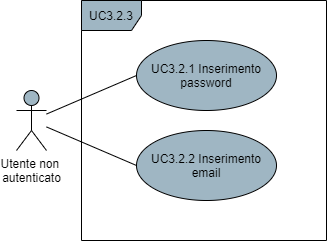
\includegraphics[scale=0.6]{res/UseCase/Immagini/InserimentoDatiLoginCliente}
\caption{Diagramma UML per UC3.2.3 - Inserimento dati login cliente}
\end{figure}

\subsubsection{UC3.2.3 - Inserimento dati login cliente}
\begin{itemize}
\item \textbf{Attori primari}: utente non autenticato;
\item \textbf{Descrizione}: l'utente compila il form per il login;
\item \textbf{Scenario Principale}: l'utente che ha selezionato il tipo utente 'cliente' \textbf{[UC3.1]} inserisce nel form apposito la propria email \textbf{[UC3.2.2]} e la propria password \textbf{[UC3.2.1]};
\item \textbf{Precondizione}: il form di inserimento dati per il login è disponibile;
\item \textbf{Postcondizione}: i dati necessari al login sono stati compilati.
\end{itemize}

\begin{figure}[H]
\centering
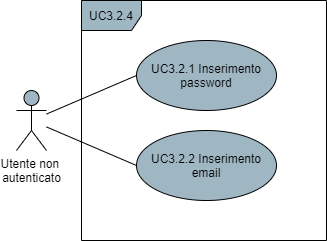
\includegraphics[scale=0.6]{res/UseCase/Immagini/InserimentoDatiLoginVenditore}
\caption{Diagramma UML per UC3.2.4 - Inserimento dati login venditore}
\end{figure}

\subsubsection{UC3.2.4 - Inserimento dati login venditore}
\begin{itemize}
\item \textbf{Attori primari}: utente non autenticato;
\item \textbf{Descrizione}: l'utente compila il form per il login;
\item \textbf{Scenario Principale}: l'utente che ha selezionato il tipo utente 'venditore' \textbf{[UC3.1]} inserisce nel form apposito la propria password \textbf{[UC3.2.1]};
\item \textbf{Precondizione}: il form di inserimento dati per il login è disponibile;
\item \textbf{Postcondizione}: i dati necessari al login sono stati compilati.
\end{itemize}

\subsubsection{UC3.3 - Richiesta di login}
\begin{itemize}
\item \textbf{Attori primari}: utente non autenticato;
\item \textbf{Descrizione}: l'utente richiede l'autenticazione con i dati inseriti;
\item \textbf{Scenario Principale}: l'utente preme il tasto di login e manda la richiesta al sistema con i dati presenti nel form;
\item \textbf{Precondizione}: l'utente prova ad autenticarsi alla piattaforma;
\item \textbf{Postcondizione}: la richiesta di login è stata mandata al sistema.
\end{itemize} 

\subsubsection{UC4 - Visualizzazione errore dati login errati}
\begin{itemize}
\item \textbf{Attori primari}: utente non autenticato;
\item \textbf{Attori secondari}: identity manager;
\item \textbf{Descrizione}: l'utente visualizza un messaggio di errore che lo informa che i dati da lui inseriti durante il login non sono riconosciuti dall'identity manager;
\item \textbf{Scenario Principale}: l'utente tenta di effettuare il login usando credenziali non presenti nel sistema;
\item \textbf{Precondizione}: l'utente prova ad autenticarsi alla piattaforma;
\item \textbf{Postcondizione}: viene visualizzato un messaggio che informa l'utente dell'errore di riconoscimento delle credenziali.
\end{itemize}

\begin{figure}[H]
\centering
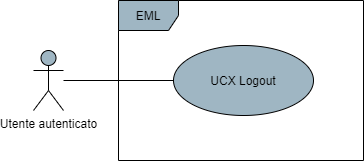
\includegraphics[scale=0.6]{res/UseCase/Immagini/Logout}
\caption{Diagramma UML per modulo di Logout}
\end{figure}

\subsubsection{UC5 - Logout}
\begin{itemize}
\item \textbf{Attori primari}: utente autenticato;
\item \textbf{Descrizione}: l'utente viene sloggato dalla piattaforma;
\item \textbf{Scenario Principale}: l'utente richiede il logout tramite il bottone dedicato;
\item \textbf{Precondizione}: l'utente ha precedentemente effettuato il login ed è attualmente autenticato;
\item \textbf{Postcondizione}: l'utente non è più autenticato.
\end{itemize}
\subsubsection{UC6.1 - Visualizzazione prodotti nel carrello}
\begin{itemize}
\item \textbf{Attori primari}: utente generico;
\item \textbf{Descrizione}: l'utente generico visualizza una lista di prodotti precedentemente inseriti nel carrello;
\item \textbf{Scenario Principale}: l'utente generico si trova nella pagina del carrello e visualizza i seguenti dati per ogni prodotto inserito nel carrello:
\begin{itemize}
\item nome del prodotto;
\item immagine del prodotto;
\item quantità presente nel carrello;
\item costo del prodotto.
\end{itemize}
\item \textbf{Precondizione}: l'utente generico si trova nella pagina del carrello;
\item \textbf{Postcondizione}: viene visualizzata la lista di prodotti presenti nel carrello.
\end{itemize}

\subsubsection{UC6.2 - Rimozione prodotto nel carrello}
\begin{itemize}
\item \textbf{Attori primari}: utente generico;
\item \textbf{Descrizione}: l'utente generico può rimuovere un prodotto precedentemente inserito nel carrello;
\item \textbf{Scenario Principale}: l'utente generico si trova nella pagina del carrello e clicca un tasto dedicato per rimuovere un prodotto dal carrello;
\item \textbf{Precondizione}: l'utente generico si trova nella pagina del carrello e ha almeno un prodotto al suo interno;
\item \textbf{Postcondizione}: il prodotto rimosso non è più presente nel carrello.
\end{itemize}

\subsubsection{UC6.3 - Modifica quantità di un prodotto nel carrello}
\begin{itemize}
\item \textbf{Attori primari}: utente generico;
\item \textbf{Descrizione}: l'utente generico può modificare la quantità di un prodotto precedentemente inserito nel carrello;
\item \textbf{Scenario Principale}: l'utente generico si trova nella pagina del carrello e clicca dei tasti dedicati per modificare la quantità di un prodotto, incrementandola o decrementandola;
\item \textbf{Precondizione}: l'utente generico si trova nella pagina del carrello e ha almeno un prodotto al suo interno;
\item \textbf{Postcondizione}: viene modificata la quantità di un prodotto del carrello in base all'intento dell'utente.
\end{itemize}

\subsubsection{UC7 Visualizzazione costo totale e tasse applicate}
\begin{itemize}
\item \textbf{Attori primari}: utente generico;
\item \textbf{Descrizione}: l'utente generico visualizza le tasse applicate e il costo totale dei prodotti nel suo carrello;
\item \textbf{Scenario Principale}: l'utente generico si trova nella pagina del carrello e visualizza il costo totale e le tasse applicate ad essi;
\item \textbf{Precondizione}: l'utente generico si trova nella pagina del carrello e ha almeno un prodotto al suo interno;
\item \textbf{Postcondizione}: viene visualizzato il costo totale dei prodotti del carrello e le tasse applicate.
\end{itemize}





\subsubsection{UC8 - Acquisto prodotti}
\begin{itemize}
\item \textbf{Attori primari}: cliente;
\item \textbf{Attori secondari}: Stripe\ped{G};
\item \textbf{Descrizione}: il cliente può acquistare i prodotti presenti nel suo carrello;
\item \textbf{Scenario Principale}: 
\begin{enumerate}
	\item il cliente inizia la procedura di checkout per i prodotti presenti nel carrello \textbf{[UC8.1]};
	\item il cliente conferma l'indirizzo email e inserisce i dati per il pagamento \textbf{[UC8.3]};
	\item il cliente procede al pagamento \textbf{[UC8.4]};
	\item il cliente visualizza un riepilogo dell'ordine effettuato \textbf{[UC8.7]}.
\end{enumerate}
\item \textbf{Precondizione}: l'utente è autenticato come cliente, si trova nella pagina del carrello e ha precedentemente inserito dei prodotti nel carrello;
\item \textbf{Postcondizione}: il costo totale dei prodotti acquistati è stato prelevato dal conto specificato dal cliente. È stata inviata un'email al cliente per confermare l'acquisto.
\end{itemize}

\begin{figure}[H]
\centering
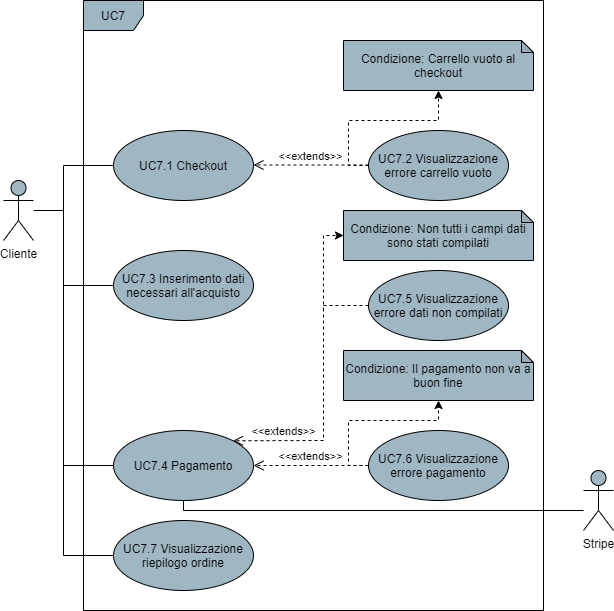
\includegraphics[scale=0.6]{res/UseCase/Immagini/AcquistoProdotti}
\caption{Diagramma UML\ped{G} per UC8 - Acquisto prodotti}
\end{figure}

\subsubsection{UC8.1 - Accesso al checkout}
\begin{itemize}
\item \textbf{Attori primari}: cliente;
\item \textbf{Descrizione}: il cliente inizia la procedura di checkout;
\item \textbf{Scenario Principale}: il cliente preme il bottone apposito per iniziare il checkout, nella pagina del carrello;
\item \textbf{Estensioni}:
\begin{itemize}
\item se non è presente alcun prodotto nel carrello viene visualizzato un messaggio di errore \textbf{[UC8.2]}.
\end{itemize}
\item \textbf{Precondizione}: l'utente è autenticato come cliente, si trova nella pagina del carrello e ha premuto il bottone per iniziare la procedura di acquisto;
\item \textbf{Postcondizione}: il cliente viene reindirizzato alla pagina di verifica email e di pagamento, dove può continuare l'acquisto dei prodotti.
\end{itemize}

\subsubsection{UC8.2 - Visualizzazione errore carrello vuoto}
\begin{itemize}
\item \textbf{Attori primari}: cliente;
\item \textbf{Descrizione}: il cliente visualizza un messaggio di errore che lo informa che per procedere al checkout è necessario avere almeno un prodotto nel carrello;
\item \textbf{Scenario Principale}: il cliente prova ad iniziare la procedura di checkout senza aver precedentemente inserito prodotti nel suo carrello;
\item \textbf{Precondizione}: il cliente si trova nella pagina del carrello e ha premuto il bottone  per iniziare la procedura di acquisto;
\item \textbf{Postcondizione}: viene visualizzato un messaggio che informa il cliente della necessità di avere almeno un prodotto nel carrello per iniziare il checkout.
\end{itemize}

\subsubsection{UC8.3 - Inserimento dati necessari all'acquisto}
\begin{itemize}
\item \textbf{Attori primari}: cliente;
\item \textbf{Descrizione}: il cliente compila i campi dati necessari all'acquisto dei prodotti selezionati;
\item \textbf{Scenario Principale}: il cliente si trova nella pagina di pagamento e, per concludere l'acquisto:
\begin{itemize}
	\item conferma l'indirizzo email indicato in fase di registrazione \textbf{[UC8.3.1]} o può indicarne uno diverso per l'invio dei prodotti acquistati \textbf{[UC8.3.2]};
	\item inserisce i dati relativi al metodo di pagamento, come nome, cognome e numero di carta di credito \textbf{[UC8.3.3]}.
\end{itemize}
\item \textbf{Precondizione}: il cliente ha iniziato la procedura di acquisto e si trova nella pagina di pagamento;
\item \textbf{Postcondizione}: il cliente può continuare il pagamento e l'acquisto.
\end{itemize}

\begin{figure}[H]
\centering
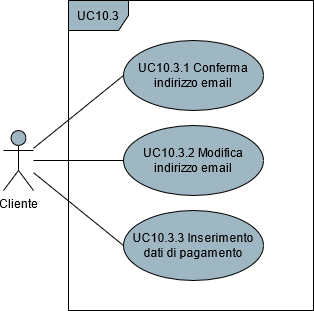
\includegraphics[scale=0.6]{res/UseCase/Immagini/InserimentoDatiAcquisto}
\caption{Diagramma UML\ped{G} per UC8.3 - Inserimento dati necessari all'acquisto}
\end{figure}

\subsubsection{UC8.3.1 - Conferma indirizzo email}
\begin{itemize}
\item \textbf{Attori primari}: cliente;
\item \textbf{Descrizione}: il cliente visualizza l'indirizzo email collegato all'account.
\item \textbf{Scenario Principale}: il cliente visualizza l'indirizzo email inserito in fase di registrazione e verifica se è effettivamente l'indirizzo sul quale vuole ricevere i prodotti acquistati. Se necessario, il cliente può modificarlo specificando un indirizzo email diverso \textbf{[UC8.3.2]};
\item \textbf{Precondizione}:  il cliente ha iniziato la procedura di acquisto e si trova nella pagina di pagamento;
\item \textbf{Postcondizione}: il cliente visualizza e conferma il suo indirizzo email.
\end{itemize}

\subsubsection{UC8.3.2 - Modifica indirizzo email}
\begin{itemize}
\item \textbf{Attori primari}: cliente;
\item \textbf{Descrizione}: il cliente modifica l'indirizzo email inserito durante la fase di registrazione;
\item \textbf{Scenario Principale}: il cliente può modificare l'email per l'invio dei prodotti, sovrascrivendo l'indirizzo visualizzato \textbf{[UC8.3.1]};
\item \textbf{Precondizione}:  il cliente ha iniziato la procedura di acquisto, si trova nella pagina di pagamento e visualizza il campo dati dedicato alla verifica dell'indirizzo email \textbf{[UC8.3.1]};
\item \textbf{Postcondizione}: il cliente modifica il suo indirizzo email, sovrascrivendo quello visualizzato.
\end{itemize}

\subsubsection{UC8.3.3 - Inserimento dati di pagamento}
\begin{itemize}
\item \textbf{Attori primari}: cliente;
\item \textbf{Descrizione}: il cliente inserisce i dati relativi alla sua carta di pagamento;
\item \textbf{Scenario Principale}: il cliente inserisce nel form relativo ai dati di pagamento le seguenti informazioni:
\begin{itemize}
	\item nome collegato al conto \textbf{[UC8.3.3.1]};
	\item cognome collegato al conto \textbf{[UC8.3.3.2]};
	\item numero di carta \textbf{[UC8.3.3.3]};
	\item mese e anno di scadenza della carta \textbf{[UC8.3.3.4]};
	\item codice di sicurezza \textbf{[UC8.3.3.5]};
\end{itemize}
\item \textbf{Precondizione}: il cliente ha iniziato la procedura di acquisto e si trova nella pagina di pagamento;
\item \textbf{Postcondizione}: il cliente ha compilato i dati di pagamento.
\end{itemize}

\begin{figure}[H]
\centering
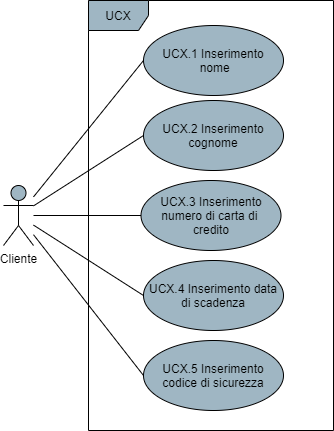
\includegraphics[scale=0.6]{res/UseCase/Immagini/InserimentoDatiPagamento}
\caption{Diagramma UML\ped{G} per UC8.3.3 - Inserimento dati di pagamento}
\end{figure}

\subsubsection{UC8.3.3.1 - Inserimento nome}
\begin{itemize}
\item \textbf{Attori primari}: cliente;
\item \textbf{Descrizione}: il cliente inserisce nelle informazioni richieste per il pagamento il nome;
\item \textbf{Scenario Principale}: il cliente inserisce nel form relativo ai dati di pagamento il nome collegato al conto;
\item \textbf{Precondizione}: il cliente ha iniziato la procedura di acquisto e si trova nella pagina di pagamento;
\item \textbf{Postcondizione}: il cliente ha compilato il campo dati dedicato al nome.
\end{itemize}

\subsubsection{UC8.3.3.2 - Inserimento cognome}
\begin{itemize}
\item \textbf{Attori primari}: cliente;
\item \textbf{Descrizione}: il cliente inserisce nelle informazioni richieste per il pagamento il cognome;
\item \textbf{Scenario Principale}: il cliente inserisce nel form relativo ai dati di pagamento il cognome collegato al conto;
\item \textbf{Precondizione}: il cliente ha iniziato la procedura di acquisto e si trova nella pagina di pagamento;
\item \textbf{Postcondizione}: il cliente ha compilato il campo dati dedicato al cognome.
\end{itemize}

\subsubsection{UC8.3.3.3 - Inserimento numero di carta di credito}
\begin{itemize}
\item \textbf{Attori primari}: cliente;
\item \textbf{Descrizione}: il cliente inserisce nelle informazioni richieste per il pagamento il numero di carta;
\item \textbf{Scenario Principale}: il cliente inserisce nel form relativo ai dati di pagamento il numero di carta di credito;
\item \textbf{Precondizione}: il cliente ha iniziato la procedura di acquisto e si trova nella pagina di pagamento;
\item \textbf{Postcondizione}: il cliente ha compilato il campo dati dedicato al numero di carta di pagamento.
\end{itemize}

\subsubsection{UC8.3.3.4 - Inserimento data di scadenza}
\begin{itemize}
\item \textbf{Attori primari}: cliente;
\item \textbf{Descrizione}: il cliente inserisce nelle informazioni richieste per il pagamento il mese e l'anno di scadenza della carta di credito;
\item \textbf{Scenario Principale}: il cliente inserisce nel form relativo ai dati di pagamento mese e l'anno di scadenza della carta;
\item \textbf{Precondizione}: il cliente ha iniziato la procedura di acquisto e si trova nella pagina di pagamento;
\item \textbf{Postcondizione}: il cliente ha compilato il campo dati dedicato alla data di scadenza.
\end{itemize}

\subsubsection{UC8.3.3.5 - Inserimento codice di sicurezza}
\begin{itemize}
\item \textbf{Attori primari}: cliente;
\item \textbf{Descrizione}: il cliente inserisce nelle informazioni richieste per il pagamento il codice di sicurezza;
\item \textbf{Scenario Principale}: il cliente inserisce nel form relativo ai dati di pagamento il codice di sicurezza collegato alla carta di credito;
\item \textbf{Precondizione}: il cliente ha iniziato la procedura di acquisto e si trova nella pagina di pagamento;
\item \textbf{Postcondizione}: il cliente ha compilato il campo dati dedicato al codice di sicurezza.
\end{itemize}

\subsubsection{UC8.4 - Pagamento}
\begin{itemize}
\item \textbf{Attori primari}: cliente;
\item \textbf{Attori secondari}: Stripe\ped{G};
\item \textbf{Descrizione}: il cliente procede all'ordine. Il pagamento viene effettuato tramite Stripe\ped{G}, che riporterà l'esito ed eventuali errori;
\item \textbf{Scenario Principale}: il cliente conferma l'ordine tramite l'apposito bottone;
\item \textbf{Estensioni}:
\begin{itemize}
	\item l'utente non ha compilato tutti i campi necessari al pagamento. Il cliente visualizza un messaggio di errore che lo informa della necessità di inserire tutti i dati per procedere al pagamento \textbf{[UC8.5]};
	\item il pagamento non va a buon fine. Il cliente visualizza un messaggio di errore contenente le cause del fallimento \textbf{[UC8.6]}.
\end{itemize}
\item \textbf{Precondizione}: il cliente si trova nella pagina di pagamento;
\item \textbf{Postcondizione}: il costo totale dei prodotti acquistati è stato prelevato dal conto specificato dal cliente. È stata inviata un'email al cliente per confermare l'acquisto. Al cliente viene mostrato un riepilogo dell'ordine appena effettuato.
\end{itemize}

\subsubsection{UC8.5 - Visualizzazione errore dati non compilati}
\begin{itemize}
\item \textbf{Attori primari}: cliente;
\item \textbf{Descrizione}: il cliente visualizza un messaggio di errore che lo informa della necessità di compilare tutti i campi dati per procedere al pagamento;
\item \textbf{Scenario Principale}: il cliente preme il bottone dedicato al pagamento senza prima aver compilato tutti i campi richiesti;
\item \textbf{Precondizione}: il cliente si trova nella pagina di pagamento e non ha compilato tutti i campi dati necessari per procedere all'acquisto;
\item \textbf{Postcondizione}: viene visualizzato un messaggio che informa il cliente dell'errore e che consiglia all'utente di controllare i dati inseriti e riprovare.
\end{itemize}

\subsubsection{UC8.6 - Visualizzazione errore pagamento}
\begin{itemize}
\item \textbf{Attori primari}: cliente;
\item \textbf{Attori secondari}: Stripe\ped{G};
\item \textbf{Descrizione}: il cliente visualizza un messaggio di errore che lo informa del motivo per il fallimento del pagamento. L'utente può poi controllare i dati inseriti e ritentare il pagamento;
\item \textbf{Scenario Principale}: il cliente prova ad effettuare il pagamento inserendo dati di una carta che per qualche motivo rifiuta l'addebito;
\item \textbf{Precondizione}: il cliente si trova nella pagina di pagamento e ha compilato i campi dati necessari per procedere all'acquisto;
\item \textbf{Postcondizione}: viene visualizzato un messaggio che informa il cliente dell'errore avvenuto nel processo di pagamento, consigliandogli di controllare i dati inseriti e riprovare.
\end{itemize}


\subsubsection{UC8.7 - Visualizzazione riepilogo ordine}
\begin{itemize}
\item \textbf{Attori primari}: cliente;
\item \textbf{Descrizione}: il cliente visualizza un riepilogo dell'ordine appena effettuato contenente l'elenco di prodotti, ognuno con prezzo e quantità, il costo totale, le tasse, l'indirizzo di spedizione e la data;
\item \textbf{Scenario Principale}: il cliente ha effettuato un ordine e ne visualizza un riepilogo;
\item \textbf{Precondizione}: il cliente ha completato un ordine ed il pagamento è andato a buon fine;
\item \textbf{Postcondizione}: viene visualizzato un riepilogo dell'ordine effettuato.
\end{itemize}

\begin{figure}[H]
\centering
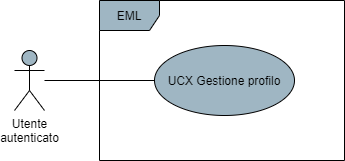
\includegraphics[scale=0.6]{res/UseCase/Immagini/ProfiloGenerale}
\caption{Diagramma UML per modulo del profilo}
\end{figure}

\subsubsection{UCX - Gestione profilo}
\begin{itemize}
\item \textbf{Attori primari}:
\item \textbf{Attori secondari}:
\item \textbf{Descrizione}:
\item \textbf{Scenario Principale}:
\item \textbf{Estensioni}:
\item \textbf{Specializzazioni}:
\item \textbf{Precondizione}:
\item \textbf{Postcondizione}:
\end{itemize}

\begin{figure}[H]
\centering
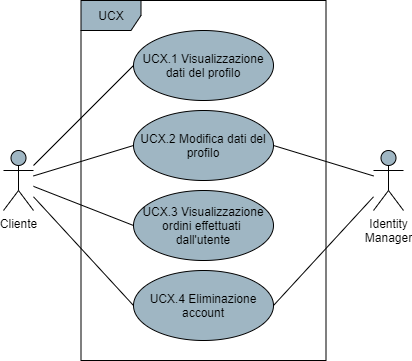
\includegraphics[scale=0.6]{res/UseCase/Immagini/GestioneProfilo}
\caption{Diagramma UML per UCX - Gestione profilo}
\end{figure}

\subsubsection{UCX.1 - Visualizzazione dati del profilo}
\begin{itemize}
\item \textbf{Attori primari}:
\item \textbf{Attori secondari}:
\item \textbf{Descrizione}:
\item \textbf{Scenario Principale}:
\item \textbf{Estensioni}:
\item \textbf{Specializzazioni}:
\item \textbf{Precondizione}:
\item \textbf{Postcondizione}:
\end{itemize}

\subsubsection{UCX.2 - Modifica dati del profilo}
\begin{itemize}
\item \textbf{Attori primari}:
\item \textbf{Attori secondari}:
\item \textbf{Descrizione}:
\item \textbf{Scenario Principale}:
\item \textbf{Estensioni}:
\item \textbf{Specializzazioni}:
\item \textbf{Precondizione}:
\item \textbf{Postcondizione}:
\end{itemize}

\subsubsection{UCX.3 - Visualizzazione ordini effettuati dall'utente}
\begin{itemize}
\item \textbf{Attori primari}:
\item \textbf{Attori secondari}:
\item \textbf{Descrizione}:
\item \textbf{Scenario Principale}:
\item \textbf{Estensioni}:
\item \textbf{Specializzazioni}:
\item \textbf{Precondizione}:
\item \textbf{Postcondizione}:
\end{itemize}

\begin{figure}[H]
\centering
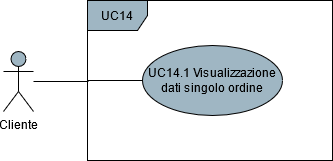
\includegraphics[scale=0.6]{res/UseCase/Immagini/VisualizzazioneOrdini}
\caption{Diagramma UML per UCX.3 - Visualizzazione ordini effettuati dall'utente}
\end{figure}

\subsubsection{UCX.3.1 - Visualizzazione dati singolo ordine}
\begin{itemize}
\item \textbf{Attori primari}:
\item \textbf{Attori secondari}:
\item \textbf{Descrizione}:
\item \textbf{Scenario Principale}:
\item \textbf{Estensioni}:
\item \textbf{Specializzazioni}:
\item \textbf{Precondizione}:
\item \textbf{Postcondizione}:
\end{itemize}

\subsubsection{UCX.4 - Eliminazione profilo}
\begin{itemize}
\item \textbf{Attori primari}:
\item \textbf{Attori secondari}:
\item \textbf{Descrizione}:
\item \textbf{Scenario Principale}:
\item \textbf{Estensioni}:
\item \textbf{Specializzazioni}:
\item \textbf{Precondizione}:
\item \textbf{Postcondizione}:
\end{itemize}

\subsubsection{UC - Caso d'uso generico}
Figura \\
\begin{itemize}
\item \textbf{Attori primari}:
\item \textbf{Attori secondari}:
\item \textbf{Descrizione}:
\item \textbf{Scenario Principale}:
\item \textbf{Estensioni}:
\item \textbf{Specializzazioni}:
\item \textbf{Precondizione}:
\item \textbf{Postcondizione}:
\end{itemize}

\subsubsection{UC11.1 - Visualizzazione dei prodotti}
\begin{itemize}
\item \textbf{Attori primari}: utente generico;
\item \textbf{Descrizione}: l'utente può visualizzare un insieme di prodotti raggruppati per categoria accedendo alla relativa PLP\ped{G};
\item \textbf{Scenario Principale}: l'utente visualizza i prodotti appartenenti ad una determinata categoria. Ogni prodotto listato nella PLP\ped{G} deve esporre le seguenti informazioni:
\begin{enumerate}
\item[a.] nome;
\item[b.] immagine;
\item[c.] prezzo;
\end{enumerate}
\item \textbf{Precondizione}: l'utente ha cliccato sulla PLP\ped{G} dedicata alla categoria di prodotti scelta;
\item \textbf{Postcondizione}: l'utente visualizza le informazioni relative ai prodotti listati, con le eventuali operazioni disponibili su ognuno di essi.
\end{itemize}
\subsubsection{UC11.2 - Selezione dei prodotti}
\begin{itemize}
\item \textbf{Attori primari}: utente generico;
\item \textbf{Descrizione}: l'utente può selezionare prodotti multipli presenti sulla PLP\ped{G} in modo da poterli inserire successivamente nel carrello, con una quantità selezionata pari ad 1. Per selezionare un prodotto è sufficiente cliccare sulla relativa casella di selezione;
\item \textbf{Scenario Principale}:
\begin{enumerate}
\item[a.] l'utente visualizza i prodotti presenti nella lista corrispondente ad una categoria [\textbf{UC11.1}];
\item[b.] l'utente clicca sulle caselle relative ad uno o più prodotti per selezionarli.
\end{enumerate}
\item \textbf{Precondizione}: l'utente sta visualizzando la PLP\ped{G} contenente uno o più prodotti desiderati;
\item \textbf{Postcondizione}: l'utente ha selezionato i prodotti desiderati.
\end{itemize}
\subsubsection{UC11.3 - Inserimento nel carrello dei prodotti selezionati}
\begin{itemize}
\item \textbf{Attori primari}: utente generico;
\item \textbf{Descrizione}: l'utente può inserire un prodotto presente sulla PLP\ped{G} nel carrello, con una quantità selezionata pari ad 1. Per effettuare l'azione è sufficiente cliccare sull'apposito pulsante;
\item \textbf{Scenario Principale}:
\begin{enumerate}
\item[b.] l'utente seleziona i prodotti desiderati [\textbf{UC11.2}];
\item[c.] l'utente preme il pulsante per l'inserimento del prodotto desiderato nel carrello.
\end{enumerate}
\item \textbf{Precondizione}: l'utente sta visualizzando la PLP\ped{G} contenente prodotti;
\item \textbf{Postcondizione}: l'utente ha inserito nel proprio carrello uno o più prodotti selezionati.
\end{itemize}
\subsubsection{UC11.4 - Filtraggio dei prodotti}
\begin{itemize}
\item \textbf{Attori primari}: utente generico;
\item \textbf{Descrizione}: l'utente può raffinare la propria ricerca andando a filtrare i prodotti presenti nella PLP\ped{G}. Il parametro utilizzabile per eseguire questa operazione è il prezzo;
\item \textbf{Scenario Principale}:
\begin{enumerate}
\item[a.] l'utente abilita il filtro attraverso l'apposita casella;
\item[b.] l'utente digita il prezzo minimo e il prezzo massimo ai quali è interessato;
\item[c.] l'utente applica il filtro cliccando l'apposito bottone.
\end{enumerate}
\item \textbf{Estensioni}:
\begin{itemize}
\item se non viene trovato nessun risultato compatibile con il range di prezzo inserito dall'utente viene visualizzato un messaggio di errore [\textbf{UC11.5}];
\end{itemize}
\item \textbf{Precondizione}: l'utente sta visualizzando i prodotti in vendita listati nella specifica PLP\ped{G};
\item \textbf{Postcondizione}: l'utente ottiene una nuova pagina in cui può visualizzare solo i prodotti presenti nella PLP\ped{G} corrente e compresi nel range di prezzo specificato.
\end{itemize}
\subsubsection{UC11.5 - Visualizzazione errore nessun risultato filtraggio}
\begin{itemize}
\item \textbf{Attori primari}: utente generico;
\item \textbf{Descrizione}: l'utente visualizza un messaggio di errore che lo informa che il filtraggio dei prodotti effettuato utilizzando i parametri da lui inseriti non ha prodotto nessun risultato.
\item \textbf{Scenario Principale}: l'utente effettua un filtraggio sul catalogo digitale selezionando un range di prezzo nel quale non è presente nessun prodotto;
\item \textbf{Precondizione}: l'utente ha effettuato l'operazione di filtraggio nella corrente PLP\ped{G};
\item \textbf{Postcondizione}: viene visualizzato un messaggio che informa l'utente di non aver trovato prodotti compatibili con quanto stabilito attraverso il range di prezzo.
\end{itemize}
\begin{figure}[H]
\centering
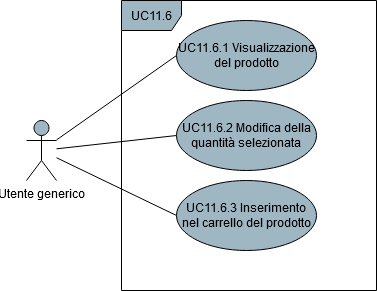
\includegraphics[scale=0.6]{res/UseCase/Immagini/VisualizzazionePaginaProdotto}
\caption{Diagramma UML per UC11.4 - Visualizzazione pagina del prodotto}
\end{figure}
\subsubsection{UC11.6 - Visualizzazione pagina del prodotto}
\begin{itemize}
\item \textbf{Attori primari}: utente generico;
\item \textbf{Descrizione}: l'utente può accedere ad una pagina per visualizzare tutte le caratteristiche di un prodotto listato. In questa pagina, chiamata anche PDP\ped{G}, è possibile eventualmente aggiungere il prodotto al carrello.
\item \textbf{Scenario Principale}: l'utente clicca sul prodotto da lui desiderato;
\item \textbf{Precondizione}: l'utente si trova in una PLP\ped{G} contenente una lista di prodotti;
\item \textbf{Postcondizione}: l'utente accede alla PDP\ped{G} corrispondente al prodotto desiderato.
\end{itemize}
\subsubsection{UCX.4.1 - Visualizzazione del prodotto}
Figura \\
\begin{itemize}
\item \textbf{Attori primari}: utente generico;
\item \textbf{Descrizione}: l'utente può visualizzare le seguenti informazioni che caratterizzano il prodotto:
\begin{itemize}
\item nome;
\item immagine;
\item descrizione;
\item prezzo;
\item tasse applicate;
\item quantità di prodotto selezionata (la quantità di default corrisponde ad 1).
\end{itemize}
\item \textbf{Scenario Principale}: l'utente visualizza le caratteristiche dell'oggetto descritto nella corrente PDP\ped{G};
\item \textbf{Precondizione}: l'utente ha cliccato sulla PDP\ped{G} dedicata al prodotto scelto;
\item \textbf{Postcondizione}: l'utente visualizza le informazioni relative ai prodotto desiderato, con la possibilità di aggiungerlo al carrello.
\end{itemize}
\subsubsection{UCX.4.2 - Modifica della quantità selezionata}
Figura \\
\begin{itemize}
\item \textbf{Attori primari}: utente generico;
\item \textbf{Descrizione}: l'utente può modificare la quantità selezionata del prodotto, che di default è 1, modificando il campo apposito;
\item \textbf{Scenario Principale}: l'utente modifica la quantità selezionata del prodotto utilizzando l'apposito campo;
\item \textbf{Precondizione}: l'utente sta visualizzando il prodotto descritto nella PDP\ped{G};
\item \textbf{Postcondizione}: la quantità del prodotto visualizzato dall'utente è stata aggiornata al nuovo valore richiesto.
\end{itemize}
\subsubsection{UCX.4.3 - Inserimento nel carrello del prodotto visualizzato}
Figura \\
\begin{itemize}
\item \textbf{Attori primari}: utente generico;
\item \textbf{Descrizione}: l'utente può inserire il prodotto nel carrello, nella quantità desiderata, cliccando un apposito pulsante. La quantità di default del prodotto corrisponde ad 1;
\item \textbf{Scenario Principale}:
\begin{enumerate}
\item[a.] l'utente visualizza le informazioni del prodotto [UC specifico];
\item[b.] l'utente può modificare la quantità del prodotto attraverso un apposito campo; [UC specifico]
\item[c.] l'utente preme il pulsante per l'inserimento del prodotto nel carrello.
\end{enumerate}
\item \textbf{Precondizione}: l'utente sta visualizzando le caratteristiche del prodotto presente nel catalogo digitale;
\item \textbf{Postcondizione}: l'utente ha inserito nel carrello il prodotto nella quantità da lui desiderata.
\end{itemize}

\begin{figure}[H]
\centering
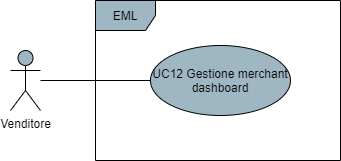
\includegraphics[scale=0.6]{res/UseCase/Immagini/MerchantDashboardGenerale}
\caption{Diagramma UML per modulo di merchant dashboard}
\end{figure}

\subsubsection{UC12 - Merchant dashboard}
\begin{itemize}
\item \textbf{Attori primari}: venditore;
\item \textbf{Descrizione}: la merchant dashboard permette di gestire e monitorare i dati dei prodotti e le vendite effettuate;
\item \textbf{Scenario Principale}: il venditore accede alla dashboard tramite l'apposito pulsante e può effettuare le seguenti operazioni:
\begin{itemize}
	\item Gestire i prodotti;
	\item Gestire le categorie di prodotti;
	\item Visualizzare gli ordini ricevuti;
	\item Visualizzare i collegamenti agli strumenti per la gestione del sito.
\end{itemize}
\item \textbf{Precondizione}: l'utente ha eseguito il login, è riconosciuto come venditore e si trova nella merchant dashboard;
\item \textbf{Postcondizione}: al merchant è permesso effettuare operazioni per gestire i propri prodotti, le categorie di prodotti e gli ordini. Sono anche presenti dei collegamenti agli strumenti di gestione del sito.
\end{itemize}

\begin{figure}[H]
\centering
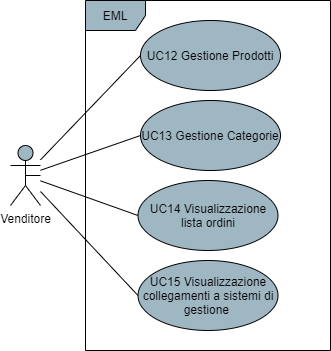
\includegraphics[scale=0.6]{res/UseCase/Immagini/MerchantDashboard}
\caption{Diagramma UML per UC12 - Merchant dashboard}
\end{figure}

\subsubsection{UC12.1 - Gestione prodotti}
\begin{itemize}
\item \textbf{Attori primari}: venditore;
\item \textbf{Descrizione}: il venditore può gestire i prodotti dalla dashboard;
\item \textbf{Scenario Principale}: il venditore può effettuare le seguenti operazioni sui prodotti:
\begin{itemize}
	\item Inserimento \textbf{[UC12.1]};
	\item Visualizzazione \textbf{[UC12.2]};
	\item Modifica \textbf{[UC12.3]};
	\item Rimozione \textbf{[UC12.4]};
\end{itemize}
\item \textbf{Precondizione}: il venditore si trova nella merchant dashboard;
\item \textbf{Postcondizione}: al venditore è permesso effettuare operazioni per gestire i propri prodotti;
\end{itemize}

\begin{figure}[H]
\centering
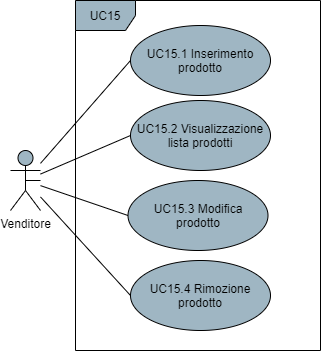
\includegraphics[scale=0.6]{res/UseCase/Immagini/GestioneProdotti}
\caption{Diagramma UML per UC12 - Merchant dashboard}
\end{figure}

\subsubsection{UC12.1.1 - Inserimento prodotto}
\begin{itemize}
\item \textbf{Attori primari}: venditore;
\item \textbf{Descrizione}: il venditore può inserire nel sistema nuovi prodotti da vendere.
\item \textbf{Scenario Principale}: il venditore accede alla pagina di inserimento prodotti tramite l'apposito pulsante ed inserisce le seguenti informazioni:
\begin{itemize}
	\item nome \textbf{[UC12.1.1]};
	\item descrizione \textbf{[UC12.1.2]};
	\item prezzo \textbf{[UC12.1.3]};
	\item immagine \textbf{[UC12.1.4]};
	\item categoria \textbf{[UC12.1.5]};
\end{itemize}
per poi premere il pulsante di conferma \textbf{[UC12.1.6]}.
\item \textbf{Precondizione}: l'utente ha eseguito il login, è riconosciuto come venditore e si trova nella merchant dashboard;
\item \textbf{Postcondizione}: il venditore ha inserito un nuovo prodotto nel sistema.
\end{itemize}

\begin{figure}[H]
\centering
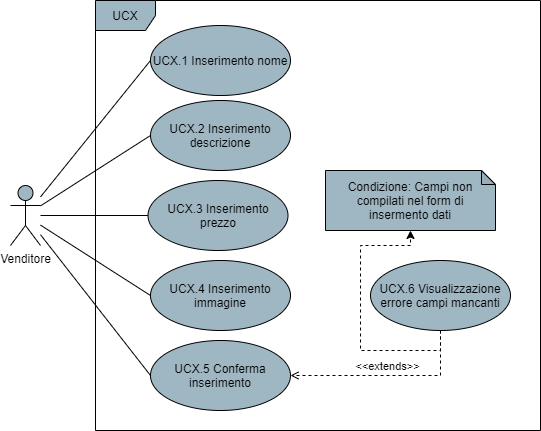
\includegraphics[scale=0.6]{res/UseCase/Immagini/InserimentoProdotto}
\caption{Diagramma UML per UC12.1 - Inserimento prodotto}
\end{figure}

\subsubsection{UC12.1.1.1 - Inserimento nome}
\begin{itemize}
\item \textbf{Attori primari}: venditore;
\item \textbf{Descrizione}: al venditore è richiesto l'inserimento del nome del nuovo prodotto da inserire;
\item \textbf{Scenario Principale}: il venditore inserisce nel form dedicato il nome del nuovo prodotto;
\item \textbf{Precondizione}: il venditore si trova nella pagina dedicata all'inserimento di un nuovo prodotto;
\item \textbf{Postcondizione}: il venditore ha compilato il campo dedicato al nome del prodotto;
\end{itemize}

\subsubsection{UC12.1.1.2 - Inserimento descrizione}
\begin{itemize}
\item \textbf{Attori primari}: venditore;
\item \textbf{Descrizione}: al venditore è richiesto l'inserimento della descrizione del nuovo prodotto da inserire;
\item \textbf{Scenario Principale}: il venditore inserisce nel form dedicato la descrizione del nuovo prodotto;
\item \textbf{Precondizione}: il venditore si trova nella pagina dedicata all'inserimento di un nuovo prodotto;
\item \textbf{Postcondizione}: il venditore ha compilato il campo dedicato alla descrizione del prodotto;
\end{itemize}

\subsubsection{UC12.1.1.3 - Inserimento prezzo}
\begin{itemize}
\item \textbf{Attori primari}: venditore;
\item \textbf{Descrizione}: al venditore è richiesto l'inserimento del prezzo del nuovo prodotto da inserire;
\item \textbf{Scenario Principale}: il venditore inserisce nel form dedicato il prezzo del nuovo prodotto;
\item \textbf{Precondizione}: il venditore si trova nella pagina dedicata all'inserimento di un nuovo prodotto;
\item \textbf{Postcondizione}: il venditore ha compilato il campo dedicato al prezzo del prodotto;
\end{itemize}

\subsubsection{UC12.1.1.4 - Inserimento immagine}
\begin{itemize}
\item \textbf{Attori primari}: venditore;
\item \textbf{Descrizione}: al venditore è richiesto l'inserimento dell'immagine del nuovo prodotto da inserire;
\item \textbf{Scenario Principale}: il venditore carica tramite tramite l'apposito bottone di upload l'immagine del nuovo prodotto;
\item \textbf{Precondizione}: il venditore si trova nella pagina dedicata all'inserimento di un nuovo prodotto;
\item \textbf{Postcondizione}: il venditore ha caricato l'immagine del nuovo prodotto;
\end{itemize}

\subsubsection{UC12.1.1.5 - Inserimento categoria}
\begin{itemize}
\item \textbf{Attori primari}: venditore;
\item \textbf{Descrizione}: al venditore è richiesto l'inserimento della categoria del nuovo prodotto da inserire;
\item \textbf{Scenario Principale}: il venditore inserisce nel form dedicato la categoria del nuovo prodotto;
\item \textbf{Precondizione}: il venditore si trova nella pagina dedicata all'inserimento di un nuovo prodotto;
\item \textbf{Postcondizione}: il venditore ha compilato il campo dedicato alla categoria del prodotto;
\end{itemize}

\subsubsection{UC12.1.1.6 - Conferma inserimento}
\begin{itemize}
\item \textbf{Attori primari}: venditore;
\item \textbf{Descrizione}: il venditore conferma i dati presenti nel form e inserisce il nuovo prodotto;
\item \textbf{Scenario Principale}: il venditore preme il pulsante di conferma e inserisce il nuovo prodotto con i dati precedentemente inseriti.
\item \textbf{Estensioni}: 
\begin{itemize}
	\item se non tutti i dati richiesti sono stati compilati viene visualizzato un messaggio di errore \textbf{[UC12.1.1.7]};
\end{itemize} 
\item \textbf{Precondizione}: il venditore si trova nella pagina dedicata all'inserimento di un nuovo prodotto e ha premuto il bottone di conferma;
\item \textbf{Postcondizione}: il venditore ha inserito un nuovo prodotto nel sistema.
\end{itemize}

\subsubsection{UC12.1.1.7 - Visualizzazione errore campi mancanti inserimento prodotto}
\begin{itemize}
\item \textbf{Attori primari}: venditore;
\item \textbf{Descrizione}: il venditore visualizza un messaggio di errore che lo informa che per procedere all'inserimento è necessario aver inserito tutti i dati richiesti;
\item \textbf{Scenario Principale}: il venditore prova ad inserire un nuovo prodotto senza aver compilato tutti i campi dati;
\item \textbf{Precondizione}: il venditore si trova nella pagina dedicata all'inserimento di un nuovo prodotto e ha premuto il bottone di conferma;
\item \textbf{Postcondizione}: viene visualizzato un messaggio che informa il venditore della necessità di compilare tutti i campi dati per completare l'inserimento di un prodotto.
\end{itemize}

\subsubsection{UC12.1.2 - Visualizzazione lista prodotti}
\begin{itemize}
\item \textbf{Attori primari}: venditore;
\item \textbf{Descrizione}: il venditore visualizza nella merchant dashboard la lista dei prodotti presenti nel sistema;
\item \textbf{Scenario Principale}: il venditore accede alla merchant dashboard e, nell'apposita sezione, visualizza nome, descrizione e immagine dei prodotti nel sistema;
\item \textbf{Precondizione}: l'utente ha eseguito il login, è riconosciuto come venditore e si trova nella merchant dashboard;
\item \textbf{Postcondizione}: il venditore visualizza la lista dei prodotti presenti nel sistema, ognuno con nome, immagine e descrizione.
\end{itemize}

\subsubsection{UC12.1.3 - Modifica prodotto}
\begin{itemize}
\item \textbf{Attori primari}: venditore;
\item \textbf{Descrizione}: il venditore può modificare i prodotti presenti nel sistema;
\item \textbf{Scenario Principale}: il venditore accede alla pagina di modifica tramite l'apposito pulsante collegato al prodotto da modificare, visualizzato nella lista dei prodotti \textbf{[UC12.1.2]}. Da li può modificare le seguenti informazioni:
\begin{itemize}
	\item nome \textbf{[UC12.1.3.1]};
	\item descrizione \textbf{[UC12.1.3.2]};
	\item prezzo \textbf{[UC12.1.3.3]};
	\item immagine \textbf{[UC12.1.3.4]};
	\item categoria \textbf{[UC12.1.3.5]}
\end{itemize}
per poi premere il pulsante di conferma \textbf{[UC12.1.3.6]};
\item \textbf{Precondizione}: l'utente ha eseguito il login, è riconosciuto come venditore e si trova nella merchant dashboard;
\item \textbf{Postcondizione}: il venditore ha modificato il prodotto selezionato.
\end{itemize}

\begin{figure}[H]
\centering
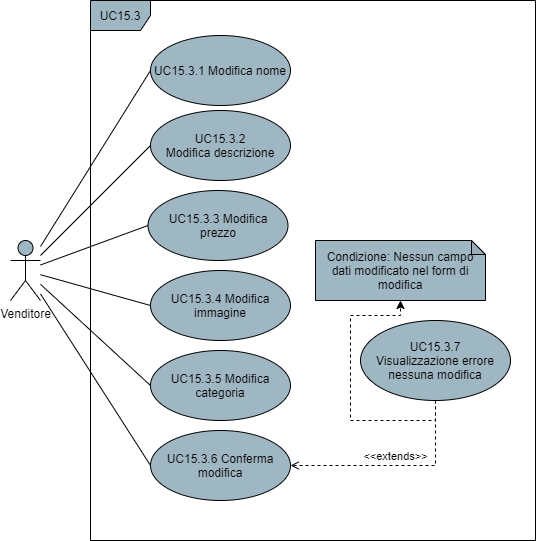
\includegraphics[scale=0.6]{res/UseCase/Immagini/ModificaProdotto}
\caption{Diagramma UML per UC12.1.3 - Modifica prodotto}
\end{figure}

\subsubsection{UC12.1.3.1 - Modifica nome}
\begin{itemize}
\item \textbf{Attori primari}: venditore;
\item \textbf{Descrizione}: il venditore modifica il nome del prodotto selezionato.
\item \textbf{Scenario Principale}: il venditore visualizza nel campo relativo al nome del prodotto il dato attualmente presente, che andrà a sovrascrivere con il nuovo nome aggiornato;
\item \textbf{Precondizione}: il venditore si trova nella pagina dedicata alla modifica di un prodotto;
\item \textbf{Postcondizione}: il venditore ha compilato il campo dedicato al nome del prodotto, sovrascrivendo il precedente;
\end{itemize}

\subsubsection{UC12.1.3.2 - Modifica descrizione}
\begin{itemize}
\item \textbf{Attori primari}: venditore;
\item \textbf{Descrizione}: il venditore modifica la descrizione del prodotto selezionato.
\item \textbf{Scenario Principale}: il venditore visualizza nel campo relativo alla descrizione del prodotto il dato attualmente presente, che andrà a sovrascrivere con la nuova descrizione aggiornata;
\item \textbf{Precondizione}: il venditore si trova nella pagina dedicata alla modifica di un prodotto;
\item \textbf{Postcondizione}: il venditore ha compilato il campo dedicato alla descrizione del prodotto, sovrascrivendo la precedente;
\end{itemize}

\subsubsection{UC12.1.3.3 - Modifica prezzo}
\begin{itemize}
\item \textbf{Attori primari}: venditore;
\item \textbf{Descrizione}: il venditore modifica il prezzo del prodotto selezionato.
\item \textbf{Scenario Principale}: il venditore visualizza nel campo relativo al prezzo del prodotto il dato attualmente presente, che andrà a sovrascrivere con il nuovo prezzo aggiornato;
\item \textbf{Precondizione}: il venditore si trova nella pagina dedicata alla modifica di un prodotto;
\item \textbf{Postcondizione}: il venditore ha compilato il campo dedicato al prezzo del prodotto, sovrascrivendo il precedente;
\end{itemize}

\subsubsection{UC12.1.3.4 - Modifica immagine}
\begin{itemize}
\item \textbf{Attori primari}: venditore;
\item \textbf{Descrizione}: il venditore modifica l'immagine del prodotto selezionato.
\item \textbf{Scenario Principale}: il venditore visualizza nel campo relativo all'immagine del prodotto quella attualmente presente, che andrà a sovrascrivere caricando la nuova immagine aggiornata;
\item \textbf{Precondizione}: il venditore si trova nella pagina dedicata alla modifica di un prodotto;
\item \textbf{Postcondizione}: il venditore ha caricato l'immagine del prodotto, sovrascrivendo la precedente;
\end{itemize}

\subsubsection{UC12.1.3.5 - Modifica categoria}
\begin{itemize}
\item \textbf{Attori primari}: venditore;
\item \textbf{Descrizione}: il venditore modifica la categoria del prodotto selezionato.
\item \textbf{Scenario Principale}: il venditore visualizza nel campo relativo alla categoria del prodotto il dato attualmente presente, che andrà a sovrascrivere con la nuova descrizione aggiornata;
\item \textbf{Precondizione}: il venditore si trova nella pagina dedicata alla modifica di un prodotto;
\item \textbf{Postcondizione}: il venditore ha compilato il campo dedicato alla categoria del prodotto, sovrascrivendo la precedente;
\end{itemize}

\subsubsection{UC12.1.3.6 - Conferma modifica}
\begin{itemize}
\item \textbf{Attori primari}: venditore;
\item \textbf{Descrizione}: il venditore conferma i dati presenti nel form e modifica il prodotto;
\item \textbf{Scenario Principale}: il venditore preme il pulsante di conferma e modifica il prodotto selezionato con i dati precedentemente inseriti.
\item \textbf{Estensioni}: 
\begin{itemize}
	\item se non viene sovrascritto nessun dato viene visualizzato un messaggio di errore \textbf{[UC12.3.7]};
\end{itemize} 
\item \textbf{Precondizione}: il venditore si trova nella pagina dedicata alla modifica di un prodotto e ha premuto il bottone di conferma;
\item \textbf{Postcondizione}: il venditore ha modificato il prodotto selezionato.
\end{itemize}

\subsubsection{UC12.1.3.7 - Visualizzazione errore nessuna modifica}
\begin{itemize}
\item \textbf{Attori primari}: venditore;
\item \textbf{Descrizione}: il venditore visualizza un messaggio di errore che lo informa che per procedere alla modifica è necessario aver sovrascritto almeno un campo dati;
\item \textbf{Scenario Principale}: il venditore prova a modificare un nuovo prodotto senza aver sovrascritto almeno un campo dati;
\item \textbf{Precondizione}: il venditore si trova nella pagina dedicata alla modifica di un prodotto e ha premuto il bottone di conferma;
\item \textbf{Postcondizione}: viene visualizzato un messaggio che informa il venditore della necessità di compilare tutti i campi dati per completare l'inserimento di un prodotto.
\end{itemize}

\subsubsection{UC12.1.4 - Rimozione prodotto}
\begin{itemize}
\item \textbf{Attori primari}: venditore;
\item \textbf{Descrizione}: il venditore può rimuovere i prodotti presenti nel sistema;
\item \textbf{Scenario Principale}: il venditore elimina il prodotto scelto tramite l'apposito pulsante collegato al prodotto da eliminare, visualizzato nella lista dei prodotti \textbf{[UC12.1.2]}.
\item \textbf{Precondizione}: l'utente ha eseguito il login, è riconosciuto come venditore e si trova nella merchant dashboard;
\item \textbf{Postcondizione}: il venditore ha eliminato il prodotto selezionato.
\end{itemize}

\subsubsection{UC12.2 - Gestione categorie di prodotti}
\begin{itemize}
\item \textbf{Attori primari}: venditore;
\item \textbf{Descrizione}: il venditore può gestire le categorie di prodotti dalla dashboard;
\item \textbf{Scenario Principale}: il venditore può effettuare le seguenti operazioni sulle categorie di prodotti:
\begin{itemize}
	\item Visualizzazione \textbf{[UC12.2.1]};
	\item Inserimento \textbf{[UC12.2.2]};
	\item Rimozione \textbf{[UC12.2.3]};
\end{itemize}
\item \textbf{Precondizione}: il venditore si trova nella merchant dashboard;
\item \textbf{Postcondizione}: al venditore è permesso effettuare operazioni per gestire le categorie di prodotti;
\end{itemize}

\begin{figure}[H]
\centering
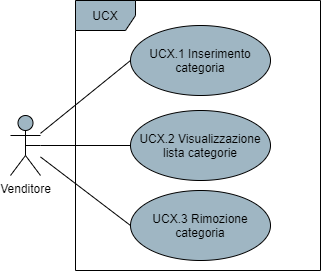
\includegraphics[scale=0.6]{res/UseCase/Immagini/GestioneCategorie}
\caption{Diagramma UML per UC12.2 - Gestione categorie di prodotti}
\end{figure}

\subsubsection{UC12.2.1 - Visualizzazione lista categorie}
\begin{itemize}
\item \textbf{Attori primari}: venditore;
\item \textbf{Descrizione}: il venditore visualizza nella merchant dashboard la lista delle categorie presenti nel sistema;
\item \textbf{Scenario Principale}: il venditore accede alla merchant dashboard e, nell'apposita sezione, visualizza una lista dei nomi delle categorie presenti;
\item \textbf{Precondizione}: l'utente ha eseguito il login, è riconosciuto come venditore e si trova nella merchant dashboard;
\item \textbf{Postcondizione}: il venditore visualizza la lista dei nomi delle categorie presenti nel sistema.
\end{itemize}

\subsubsection{UC12.2.2 - Inserimento categoria}
\begin{itemize}
\item \textbf{Attori primari}: venditore;
\item \textbf{Descrizione}: il venditore può inserire nel sistema nuove categorie di prodotti.
\item \textbf{Scenario Principale}: il venditore accede alla pagina di inserimento categorie tramite l'apposito pulsante ed inserisce il nome della categoria \textbf{[UC12.2.2.1]} per poi premere il pulsante di conferma \textbf{[UC12.2.2.2]}.
\item \textbf{Precondizione}: l'utente ha eseguito il login, è riconosciuto come venditore e si trova nella merchant dashboard;
\item \textbf{Postcondizione}: il venditore ha inserito una nuova categoria nel sistema.
\end{itemize}

\begin{figure}[H]
\centering
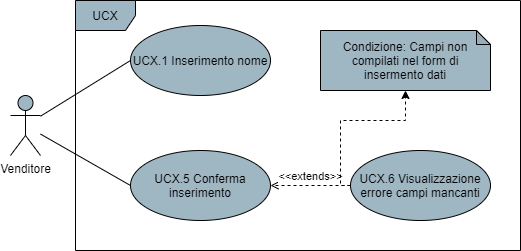
\includegraphics[scale=0.6]{res/UseCase/Immagini/InserimentoCategoria}
\caption{Diagramma UML per UC12.2.2.2 - Inserimento categoria}
\end{figure}

\subsubsection{UC12.2.2.1 - Inserimento nome}
\begin{itemize}
\item \textbf{Attori primari}: venditore;
\item \textbf{Descrizione}: al venditore è richiesto l'inserimento del nome della nuova categoria da inserire;
\item \textbf{Scenario Principale}: il venditore inserisce nel form dedicato il nome della nuova categoria;
\item \textbf{Precondizione}: il venditore si trova nella pagina dedicata all'inserimento di una nuova categoria;
\item \textbf{Postcondizione}: il venditore ha compilato il campo dedicato al nome della categoria;
\end{itemize}

\subsubsection{UC12.2.2.2 - Conferma inserimento}
\begin{itemize}
\item \textbf{Attori primari}: venditore;
\item \textbf{Descrizione}: il venditore conferma i dati presenti nel form e inserisce la nuova categoria;
\item \textbf{Scenario Principale}: il venditore preme il pulsante di conferma e inserisce la nuova categoria con il nome precedentemente inserito
\item \textbf{Estensioni}: 
\begin{itemize}
	\item se il nome della categoria non è stato inserito viene visualizzato un messaggio di errore \textbf{[UC12.2.2.3]};
\end{itemize} 
\item \textbf{Precondizione}: il venditore si trova nella pagina dedicata all'inserimento di una nuova categoria e ha premuto il bottone di conferma;
\item \textbf{Postcondizione}: il venditore ha inserito una nuova categoria nel sistema.
\end{itemize}

\subsubsection{UC12.2.2.3 - Visualizzazione errore campi mancanti inserimento categoria}
\begin{itemize}
\item \textbf{Attori primari}: venditore;
\item \textbf{Descrizione}: il venditore visualizza un messaggio di errore che lo informa che per procedere all'inserimento è necessario aver inserito il nome della categoria;
\item \textbf{Scenario Principale}: il venditore prova ad inserire una nuova categoria senza aver compilato il campo dati del nome;
\item \textbf{Precondizione}: il venditore si trova nella pagina dedicata all'inserimento di una nuova categoria e ha premuto il bottone di conferma;
\item \textbf{Postcondizione}: viene visualizzato un messaggio che informa il venditore della necessità di compilare il campo del nome per inserire una nuova categoria.
\end{itemize}

\subsubsection{UC12.2.3 - Rimozione categoria}
\begin{itemize}
\item \textbf{Attori primari}: venditore;
\item \textbf{Descrizione}: il venditore può rimuovere le categorie;
\item \textbf{Scenario Principale}: il venditore elimina la categoria scelta tramite l'apposito pulsante collegato alla categoria da eliminare, visualizzato nella lista delle categorie \textbf{[UC12.2.1]}.
\item \textbf{Precondizione}: l'utente ha eseguito il login, è riconosciuto come venditore e si trova nella merchant dashboard;
\item \textbf{Postcondizione}: il venditore ha eliminato la categoria selezionata.
\end{itemize}


\subsubsection{UC12.3 - Visualizzazione lista ordini ricevuti}
\begin{itemize}
\item \textbf{Attori primari}: venditore;
\item \textbf{Descrizione}: il venditore visualizza nella merchant dashboard la lista degli ordini ricevuti;
\item \textbf{Scenario Principale}: il venditore accede alla merchant dashboard e, nell'apposita sezione, visualizza una lista degli ordini ricevuti. Per ogni ordine viene visualizzato il numero dell'ordine, il costo totale e la data. Il venditore può accedere ad altre informazioni premendo il bottone 'Dettagli' collegato all'ordine interessato \textbf{[UC12.4]}.
\item \textbf{Precondizione}: l'utente ha eseguito il login, è riconosciuto come venditore e si trova nella merchant dashboard;
\item \textbf{Postcondizione}: il venditore visualizza la lista degli ordini presenti nel sistema.
\end{itemize}

\subsubsection{UC12.4 - Visualizzazione informazioni ordine}
\begin{itemize}
\item \textbf{Attori primari}: venditore;
\item \textbf{Descrizione}: il venditore visualizza le informazioni dell'ordine selezionato;
\item \textbf{Scenario Principale}: il venditore accede alla pagina di visualizzazione informazioni ordine tramite il pulsante 'Dettagli' collegato all'ordine selezionato nella lista degli ordini ricevuti \textbf{[UC12.3]}. In particolare vengono visualizzati i seguenti dati:
\begin{itemize}
	\item numero ordine;
	\item prodotti acquistati;
	\item quantità prodotti acquistati;
	\item costo per singola voce;
	\item costo totale;
	\item tasse applicate;
	\item data acquisto;
\end{itemize}
\item \textbf{Precondizione}: l'utente ha eseguito il login, è riconosciuto come venditore e si trova nella merchant dashboard;
\item \textbf{Postcondizione}: il venditore visualizza le informazioni relative all'ordine selezionato.
\end{itemize}

\subsubsection{UC12.5 - Collegamenti a sistemi di gestione}
\begin{itemize}
\item \textbf{Attori primari}: venditore;
\item \textbf{Descrizione}: il venditore visualizza nella merchant dashboard i collegamenti agli strumenti di gestione esterni;
\item \textbf{Scenario Principale}: il venditore accede alla merchant dashboard e, nell'apposita sezione, visualizza dei collegamenti alla piattaforma di monitoraggio dell'applicazione e agli strumenti di configurazione \textbf{[UC14]}.
\item \textbf{Precondizione}: l'utente ha eseguito il login, è riconosciuto come venditore e si trova nella merchant dashboard;
\item \textbf{Postcondizione}: il venditore visualizza la lista dei collegamenti ai sistemi di gestione del sito.
\end{itemize}

